\documentclass{article}

\usepackage[final]{style}
\usepackage[utf8]{inputenc} % allow utf-8 input
\usepackage[T1]{fontenc}    % use 8-bit T1 fonts
\usepackage{hyperref}       % hyperlinks
\usepackage{url}            % simple URL typesetting
\usepackage{booktabs}       % professional-quality tables
\usepackage{amsfonts}       % blackboard math symbols
\usepackage{nicefrac}       % compact symbols for 1/2, etc.
\usepackage{microtype}      % microtypography
\usepackage{verbatim}
\usepackage{graphicx}       % for figures
\graphicspath{ {./images/} }

\title{Lecture \#1: Introduction to Reinforcement Learning}

\author{
  Joel Lee\\
  Department of Computer Science\\
  National University of Singapore\\
  Singapore, S117417 \\
  \texttt{\{joel, STUDENT2, etc.\}@u.nus.edu} \\
}

\begin{document}

\maketitle

\section{Introduction}
Welcome to CS6101

\section{Policy for the course}
The class will meet every week around 3pm to 5pm to review the
material presented. Prof Min and Prof Lee Wee Sun will be giving
lectures for the first two weeks (Week 3, this week) and Week 4. For
subsequent weeks, participants will take turns assuming the role of
scribe/lecturer.

\section{Supervised Learning and Imitation Learning}

In Supervised learning, we train a model to match the input to other
labels, perhaps say, using mean square error or some other model to
check for accuracy or loss. In reinforcement learning, we learn and
reiterate using feedback. Given a state, we need to decide what action
we wish to take.


For greater detail, refer to
\href{https://hackernoon.com/reinforcement-learning-and-supervised-learning-a-brief-comparison-1b6d68c45ffa}{A brief comparison of reinforcement learning and supervised learning}. The goal of reinforcement learning is more general than supervised learning and we can then couple this in a sequential method to build
up a policy.


\section{States vs Observations}
We aim to learn theta which represents the weights in a deep network and models the conditional distribution over a given observation. In some reinforcement learning algorithms you learn a value function through which you can derive a policy instead of learning the function directly.
In the most general kind of view of RL your policies give you actions conditioned on observations. In fully observed settings you have actions conditioned on states.


The key difference between states and observations is that states satisfy the Markov property. That is to say, given three states, state 3 is conditionally independent of state 1 given state 2. Observations, on the other hand, do not satisfy this criteria.

In imitation learning we collected observation action tuples to train on. We then used a supervised learning algorithm that maps from observation to action


A key point of note is that we are trying to maximize the reward over all time and not the reward given the current state. For further illustration, consider the following example: You are driving a car and you get high reward for driving fast but a significant penalty when you hit another car so you might avoid driving faster at intersections because you know it might lead to states with lower rewards.




\subsection{Policy}
Given a state, what action are we going to take?

\subsection{State}
Action doesn't directly affect the policy. State is what is actually
happening in the worl.  Based on what we can see from sensory input,
we can take an action.  Tiger and the car(Observation wouldn't let us
see it). we can't observe the tiger but our previous state allows us
to know

\subsection{Markov property}
If I know the current state of the system I know whawt's the
probability of getting to the next state. Particular state + what's
the reward for taking an action.

\section{Finite horizon vs infinite Horizon}
Finite horizon is not stationary -- it diverges.
At Initial time point it may be at a stable state. Hundred or thousand points can be just of the stationary distribution.
- Reward function: Stationary distribution
- Reward function can discount rewards over time(Just ensure it is stable at the end)
- Agent falls off the cliff and breaks then th process can't be reversed.
- Ergodicity assumption doens't get us into a log of trouble
- Policy is trained on stationary distribution( Policy may not be making the most optimal move)

- Stationary distribution: Multiply against transition proba you get exact same distribution
- Infinite Horizon case: reach any state given any different state
- If there is a terminal state and a non-zero probability of transitioning to it.
- nonzero probability that it is going to a terminal state
- Probability one in the terminal state
- Reward function may not be smooth but it doesn't stop us from applying a reinforcement learning approach
- SGD must be differentiable but if you take an RL approach it doesn't need to be. Reward function doesn't need ot be smooth

- Policy gradients, fit the model.
- Loss function of how badly the agent is doing
- Take the expectation of how well the policy performs
- Whole bunch of different ways(Base/model free)

- Total reward for taking an action at a particular time at a particular state(Q value is specific to policy and it computes reward for all of the subsequent time steps)


- State of the board as you receive it as an agent
- Q-function I take one or infinite or discrete number of actions how my value function will change

- Calculate how good a particular policy is
- Value function your reward what is your best position after making a move. How likely is it for you to win? 
- Set probability to zero everywhere except for the one region where it is 
- High variance slow learning, need many samples to estimate the gradient( How do we reduce the variance)
- History/Markovian property of state
- Most of this cost(Probabilistic interpretation
- Sum of all the rewards over that particular trajectory
- Expectation over all trajectories
\section{The goal of reinforcement learning }
We want to find  parameter theta* which maximizes the expectation under the trajectory of the distribution induced by theta of the total reward of the trajectory

We write it as an expectation because in general the states and actions we see for a parameter vector are random variables and we have to take the sum of rewards in expectation

Probability of an action under the policy given past state

\section{DAGGER}
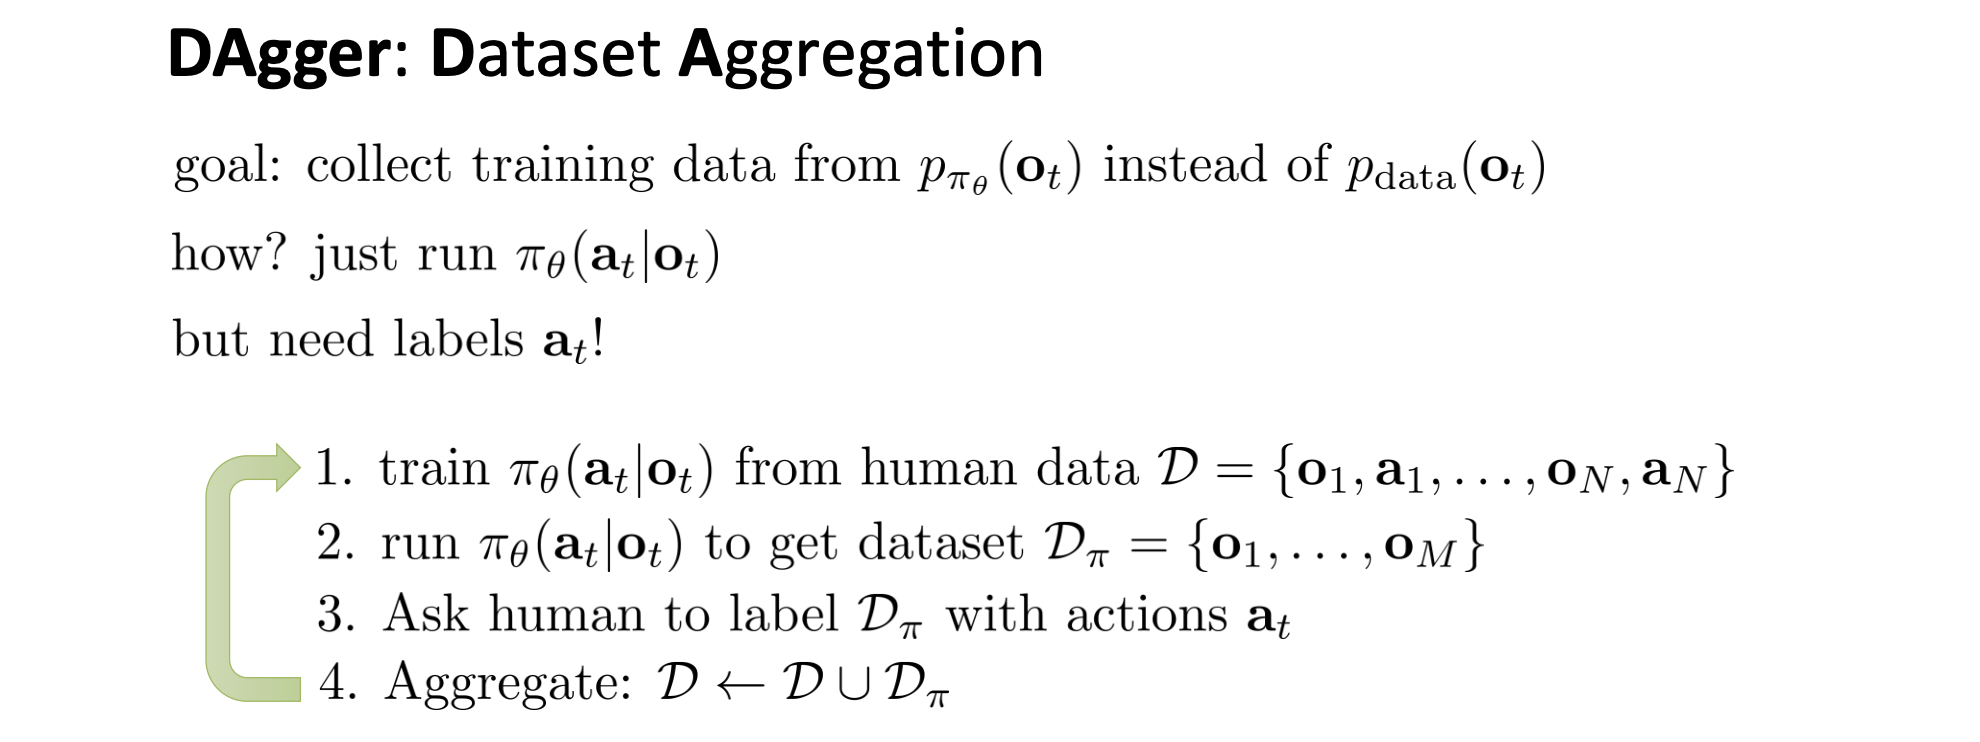
\includegraphics[scale=0.5]{dagger}

\section{REINFORCE}


\section{Definitions}


\subsection{Markov Decision Process}
A Markov Decision Process is an extension of a Markov chain. In this diagram, we have S representing the state space and T representing the transition operator. $\mu$ is a vector of five numbers that sum up to one 

Markov chains satisfy the markov property which is to say that the next state is conditionally independent given the present one.

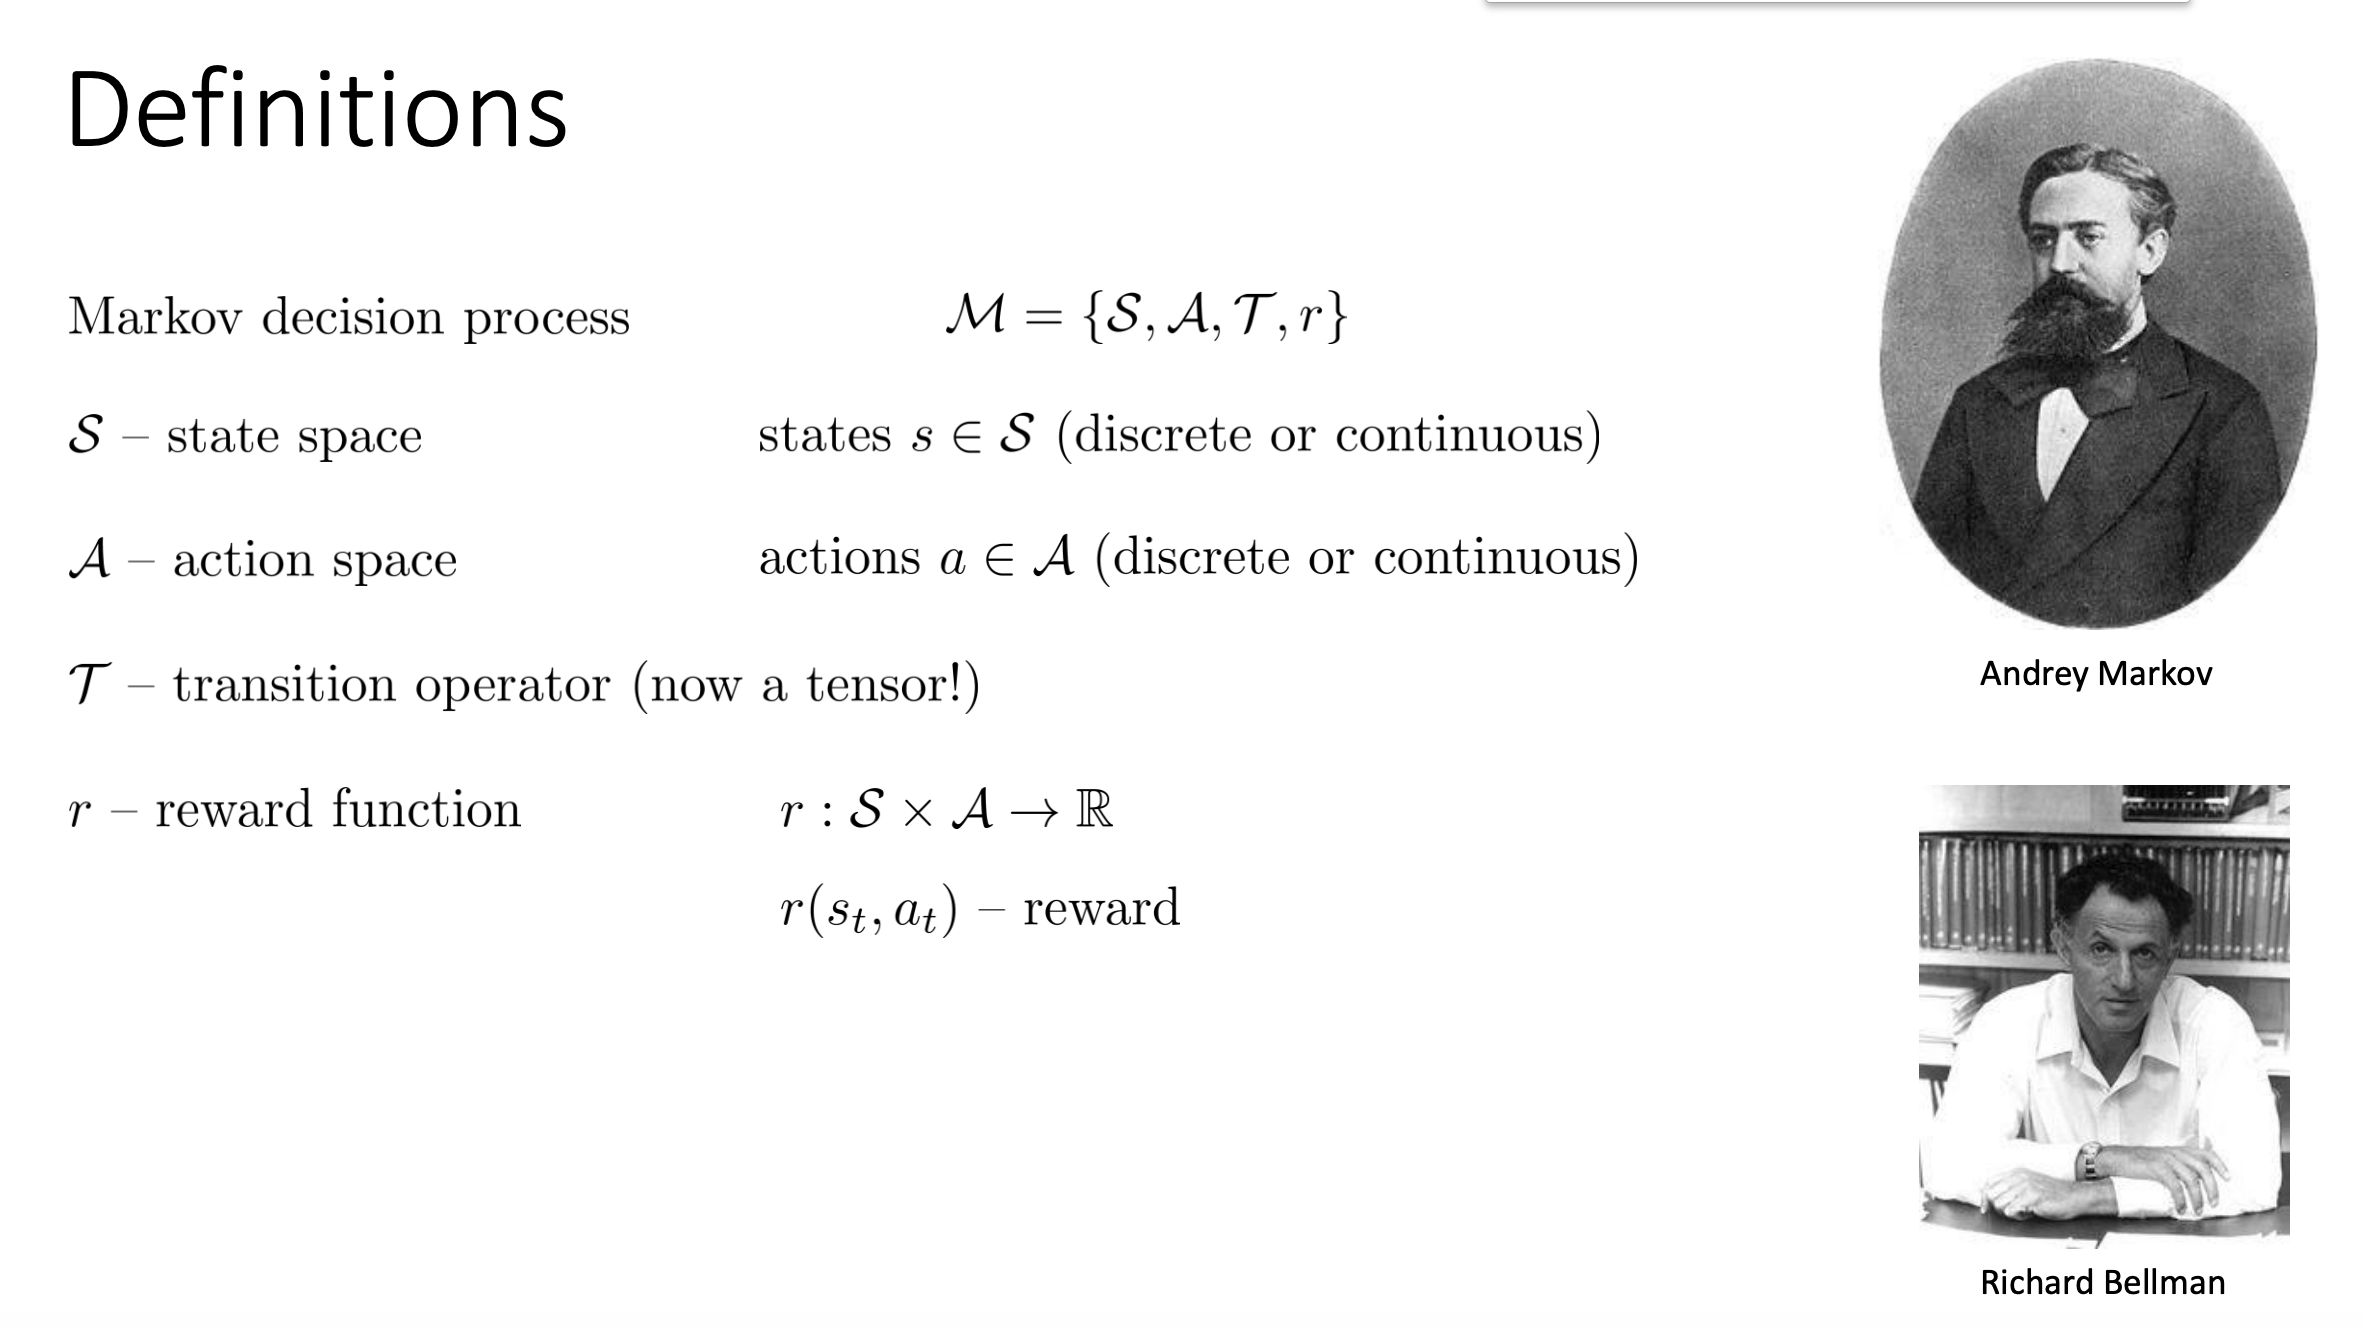
\includegraphics[scale=0.25]{mdp}

Transition operator is now a tensor which expresses that given States and actions we have a Reward function which is a scalar valued function on teh corss product of states over all the states and actions.
If we choose to act on observations without knowing what states are then we get a generalization of the MDP known as a partially observed markov decision process.


\subsection{Finite Horizon MDP}
- Finite horizon, take teh expectation outside and by linearity of expectation the thing inside the sum the reward only depends on the state and action that wtime step
We have sum over time of the reward at a time step
22:16 : State action marginal
- In the infinite horizon case does p(st, at) converge to a stationary distribution? that is to say $\mu = T * \mu$
and $(T- I) * \mu =0$

We put a 1/T in front which is supposed to be okay because dividing by that constant doesn't change the optimum

In the infinite horizon case it's just the expected reward under the stationary distribution of the markov chain

Just because you have objectives and reward functions that are not smooth it doesn't mean that the resulting reinforcement learning problem is not smooth because reinforcement learning almost always cares bout expectations


\section{Anatomy of a reinforcement learning algorithm}

Include slide at 36:23

We try to learn f-phi that predicts the next state. This is model-based RL
in this scenario we use samples ot fit fphi so that it can do a better job predicting hte next state. In blue box you backprop and update policy

Model-based only handles deterministic dynamics and deterministics policies and only continuous states and actions. So it is not enough

In order to work with stochastic systems we will introduce the notion of a value function

Easy to modify our policy if we know the Q that we defined in 48:45

Expectation of value is our RL objective~

policy(a|s) = 1 if action maximizes value of Q

then we compute gradient to increase the probability of taking the good actions a
if q $ policy(s,a) > valuepi_s$ then a is better than average

\section{Type of algorithms}
- Policy gradients(differentiate objective)
- value-based(estimate value function) or the optimal policy
- Actor-critic: estimate  value function or q-function of the current policy and use it to improve policy
- Model-based RL: Estimate the transition model

Model based rl
- Use the model to plan(no policy)
- Monte Carlo Tree Search
- Trajectory optimization/optimal control
- Backprop gradients into policy
- Use model to learn a value function via DP or Dyna(model generates synthetic experience) and this exp is plugged into a model free learner


Why do we need so many RL algos
1. Sample efficiency
2. Stability and ease of use
3. Assumptions that work only under certain scenarios

\subsection{On-Policy vs Off-Policy}
An on-policy algorithm requires that we generate new samples every time the policy is changed.

In contrast, an off-policy algorithm allows us to improve the policy without generating any new samples from the policy

Common assumptions in RL:
- observability
- episodic learning
- continuity



\section{Policy Gradients Introduction}
Define a distribution over trajectories by multiplying policy at all times step times the transition probabilities

Maximizing J(Theta)

We can convert this to integral form as in 10:12

Note the convenient identity at 11:37

Substituting into 12:12

Components in 15:25 are not affected by theta so we can cancel them out

Maximum likelihood looks like policy gradient except multiplied by total reward. This is not a conicidence you are weighting all your samples by how good they are 

\section{What is wrong with the policy gradient?}
Big positive constant can skew the curve easily. Illustrate with 29:37-ish region


Trick one to reduce variance: Future doesn't affect the past(Causality: Nothing I do right now will affect what happened ten minutes ago)

Change the equation at 37:42
This is okay because changing the policy at that particular time step is not going to change the rewards of previous time steps

This is the total reward I'll get from now until the end. It is the reward to go

This reduces variance because you sum less terms and the numbers you get are smaller and if you recall variance is squared. so you get smaller numbers just because of the decrease in magnitude

We can multiply by reward - b because we want to make things that are more rewarding than usual go up

49:22
We wish to find the optimal b such that dVar/db = 0 and we find that this occus when b=
Describe importance sampling 56:00

\section{Actor-Critic}

% References
\small
\bibliographystyle{plain}
\bibliography{bibliography}
\end{document}
